\chapter{Circuit simulations for generating various waveform signals}
Circuit simulations were run to validate the behaviour of the conceptual design and to present the trade offs.
A harmonic balance simulation was used to investigate the concepts of chapter \ref{ch:design}, as it presented a steady state solution neglecting the transient state.
This frequency domain simulation was run with the tool \gls{ab:ads} to present the solution for the nonlinear behaviour of the test circuit.
In a first step the generation of various analog output signals were investigated.
Three basic signal waveforms were synthesized to show the ability of generating different signals.
Afterwards the designed test circuit of chapter \ref{ch:design} was tested with respect to stability and its energy consumption.
As the realized circuit differed a bit from the presented test circuit in chapter \ref{ch:design}, another simulation was run to get an impression what to expect for the measurement.
The presented simulations were run with the schematic shown in appendix \ref{app:schematic}, except for the simulation of the built demonstrator in chapter \ref{ch:ProofOfConceptWithExistingComponents}.

\section{Generating various analog signals with digital input control}
Generating analog signals from a digital input signal was the aim of the presented work.
The designed custom \gls{ab:dac}, the Riemann Pump, should be able to synthesize various waveform signals at the output.
Simulation results were presented in the time domain to validate the integrity of the desired signal.
In the system design a pre processor is used to compute the Riemann Code with a specific algorithm.
For simulation purposes the digital Riemann Code was computed manually, as seen for example in Figure \ref{fig:RiemannCodeGenerationSineWave}.
A prerequisite for the design process was a resolution of the \gls{ab:dac} of three bits.
Another prerequisite was an \gls{ab:osr} of four, as discussed in chapter \ref{ch:fundamentals}.
The presented simulations of the digital-to-analog conversion were run to proof the concept of the designed test circuit.
 
\subsection{Sine wave generation in the time domain}
As known from basic signal processing, the sine wave for continuous time is the elementary signal and therefore synthesized first. 
For the generation of this sine wave a corresponding Riemann Code was required which will be converted to the desired sine wave.\\
This Riemann Code was generated by hand via an approximation of a sine wave with a sequence of eight different slopes.
Eight different slopes represented the three bit resolution while the sequence of eight sampling points represented the \gls{ab:osr} of four. 
Figure \ref{fig:RiemannCodeGenerationSineWave} illustrates this approximation to get the corresponding Riemann Code.

%\begin{figure}[htb!]
%   \centering
%   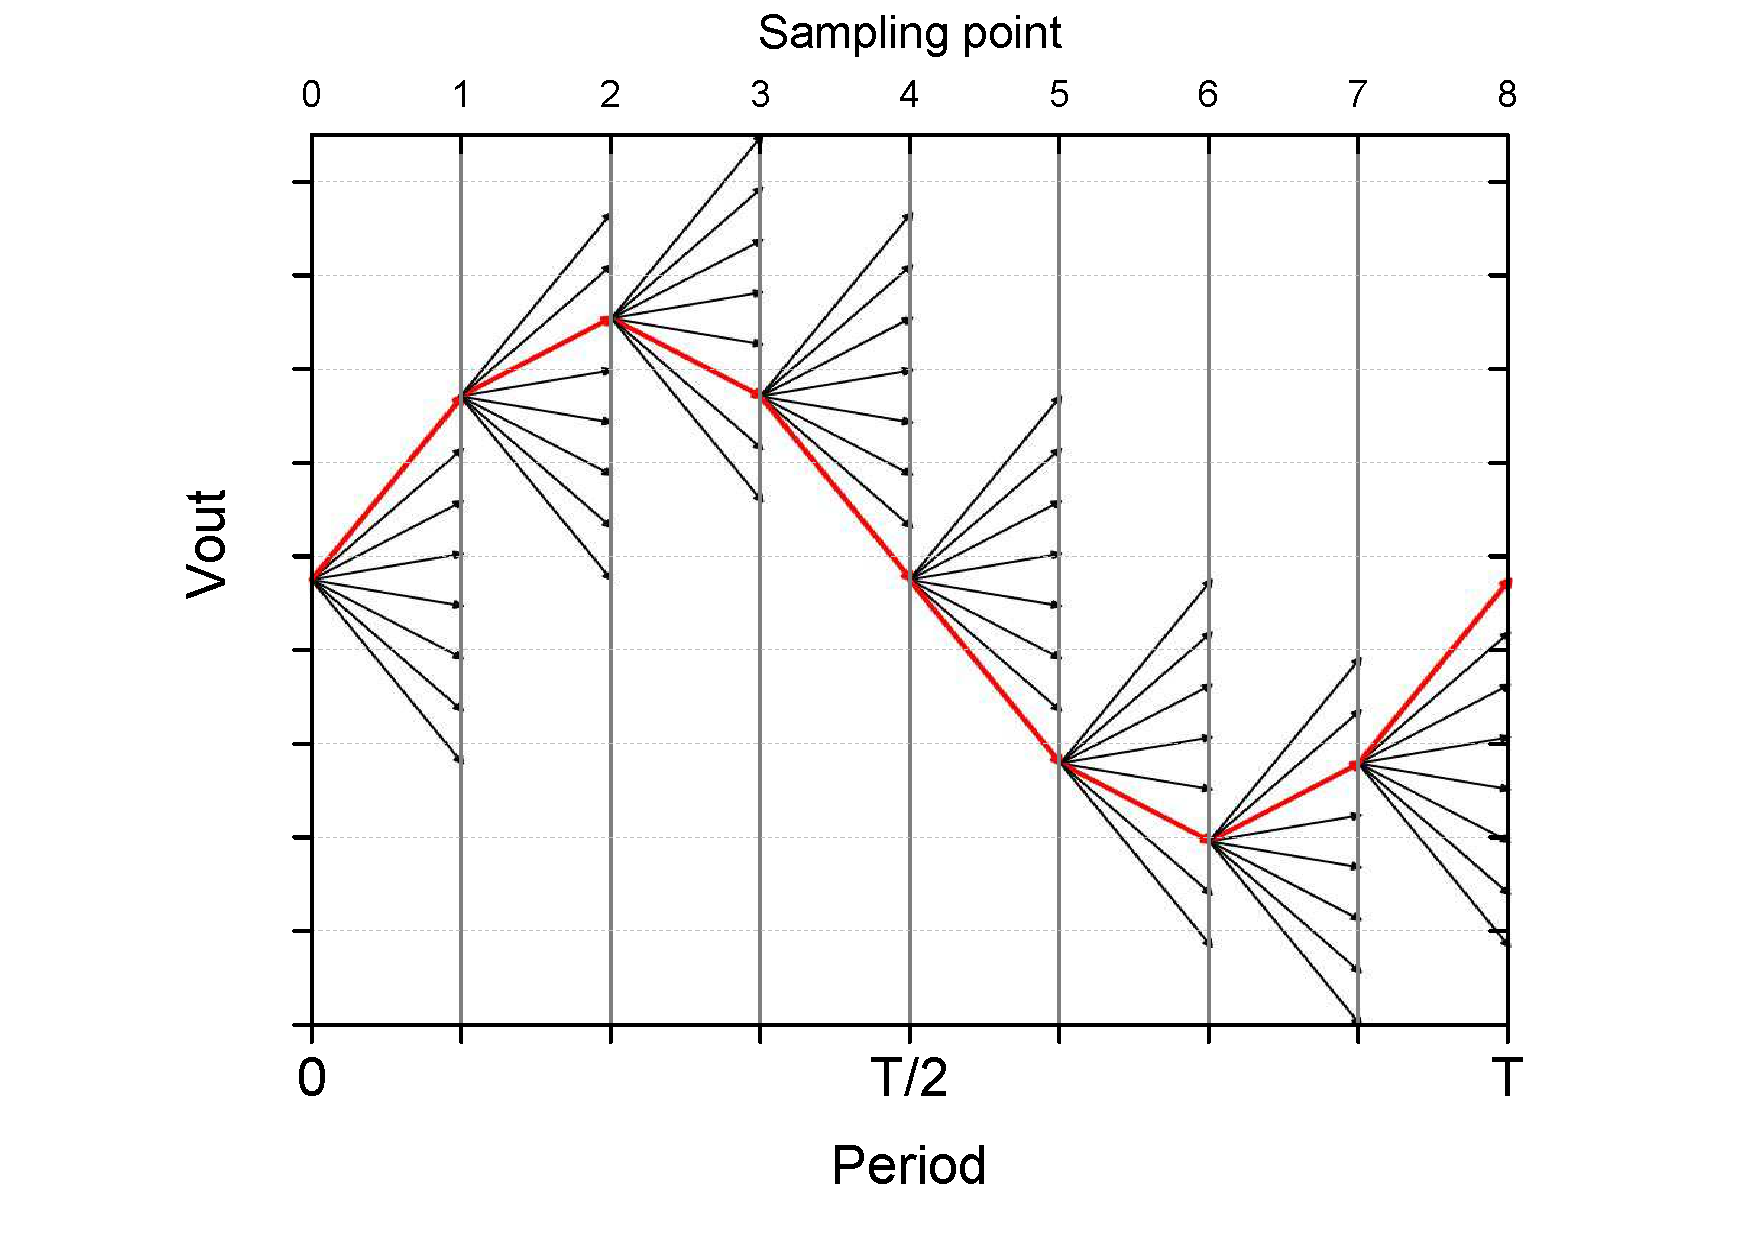
\includegraphics[width=0.75\textwidth]{RiemannCodeGeneration.pdf}
%   \caption{One possible approximation of sine wave generation to get the Riemann Code}
%   \label{fig:RiemannCodeGenerationSineWave}
%\end{figure}

%To validate the feasibility of the presented concept, a digital input control code is required.
%To get this code an approximation by hand is done since no algorithm exists which can compute this.

\begin{figure}[htb!]
   \centering 
   \input{graphics/simulation/RiemannCodeGenerationSineWave73_latest.pdf_tex}
   \caption{One possible approximation of a sine wave generation to get the Riemann Code}
   \label{fig:RiemannCodeGenerationSineWave}
\end{figure}


The sequence of chosen slopes, referred to $i_0$ values, is:
\begin{equation}
 +7\hspace{.3cm} +3\hspace{.3cm} -3\hspace{.3cm} -7\hspace{.3cm} -7\hspace{.3cm} -3\hspace{.3cm} +3\hspace{.3cm} +7,
 \end{equation} 
which represents the following encryption:
\begin{equation}
000\hspace{.3cm} 010\hspace{.3cm} 101\hspace{.3cm} 111\hspace{.3cm} 111\hspace{.3cm} 101\hspace{.3cm} 010\hspace{.3cm} 000,
\label{eq:RiemannCodeSineWave} 
\end{equation}

based on the encryption table in Figure \ref{fig:SlopesAndTable}, chapter \ref{ch:fundamentals}.
The generated Riemann Code consists of eight triplets, where each triplet represents the three bit resolution.
The quantity of digits in each set, here triplet, increases with the number of bits used for the resolution.
The number of triplets represents the number of sampling points, corresponding to the \gls{ab:osr}.
This particular generated Riemann Code in equation \ref{eq:RiemannCodeSineWave} was used to synthesize sine waves in the frequency range between \SI{500}{\MHz} and \SI{6}{\GHz}, as shown in Figure \ref{fig:7SignalsSameSlopeInOnePlot}.

%\begin{figure}[htb!]
%   \centering 
%   \input{graphics/simulation/Vout_sine_SigBWdifferent_SameSlope_73_TwoPeriods.pdf}
%   \caption{Synthesized signals with demonstrated Riemann Code for the frequency range of \SI{0.5}{\GHz} to \SI{6}{\GHz}}
%   \label{fig:7SignalsSameSlopeInOnePlot}
%\end{figure}

\begin{figure}[htb!] %% Add sampling points at the top !!
   \centering
   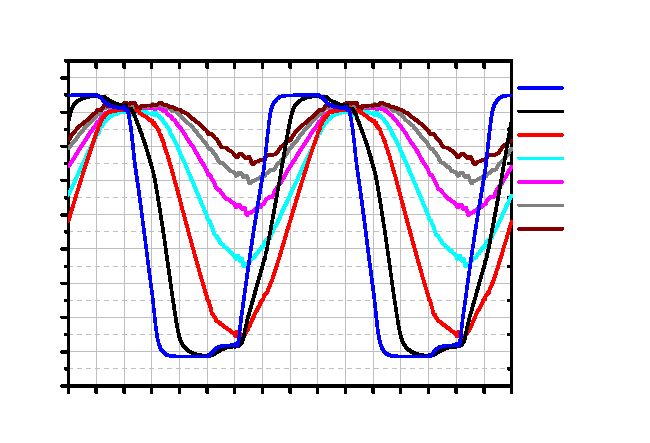
\includegraphics[width=0.75\textwidth]{Vout_sine_SigBWdifferent_SameSlope_73_TwoPeriods.pdf}
   \caption{Synthesized signals with demonstrated Riemann Code for the frequency range of \SI{0.5}{\GHz} to \SI{6}{\GHz}}
   \label{fig:7SignalsSameSlopeInOnePlot}
\end{figure}


The amplitude of seven signals with different frequencies are shown over their period while at the top the number of sampling points is shown.
This representation is chosen to compare the signal integrity of different frequencies.
The shape from most of the plotted functions fit fairly to a theoretical sine wave.
As the sampling interval differs for different frequencies, the amplitudes of the signals also differed.
The maximum reachable amplitude was the positive supply voltage, here set to \SI{15}{\volt}, while the lower bound was \SI{0}{\volt}. 
Once the amplitude reached the supply voltage, the signal wave form is clipped due to a fully charged output capacitor.
This undesired effect transformed the sine wave into a rectangular shaped signal form, as seen for the blue and black curve.
Therefore a bandwidth limitation is introduced.\\
Figure \ref{fig:7SignalsSameSlopeInOnePlot} highlights a limitation of the designed circuit as the blue curve turns into a rectangular signal form.\\

\begin{figure}[htb!] %% Add sampling points at the top !!
   \centering
   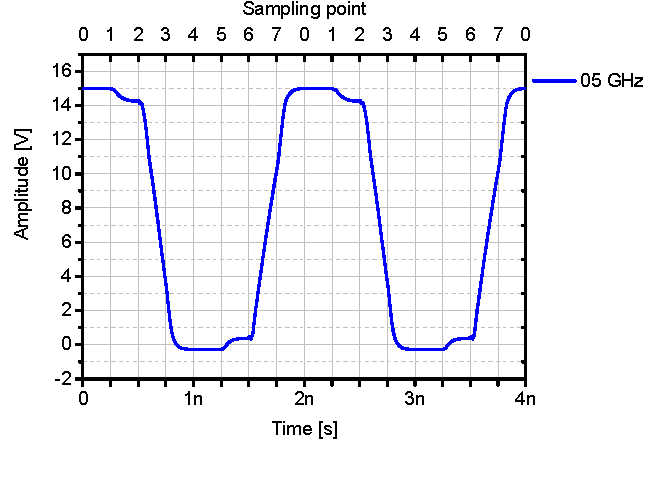
\includegraphics[width=0.75\textwidth]{Vout_sine_SigBW_05GHz_3bit_long.pdf}
   \caption{Synthesized sine wave for frequency of 0.5GHz}
   \label{fig:SineWave05GHz}
\end{figure}


Below the frequency of \SI{1}{\GHz} the desired shape of a sine wave was transformed to a rectangular  form due to the long sampling time.
In addition to the unwanted rectangular form another distortion occurred, depicted in the blue signal for the sampling interval 1 to 2 and 5 to 6.
An unsymmetrical switching process, the finite rise time of the provided current and the not perfectly defined current sources were three factors to mention. %, as the gate of the switching transistor had to be charged 
Furthermore a leakage current were induced by the commutation time of the switching process.
This distortion was mainly observed for low frequencies when the output capacitance was fully charged and discharged.
In the higher frequency range this did not effect the integrity very much.
As already mentioned in the design process, the circuit was designed to fulfil the requirement of synthesizing signals in high frequencies.\\
The signal frequency of \SI{1}{\giga \hertz} represented a lower bound on the frequency range in the used configuration. % referred to chapter \ref{ch:design} of the circuit.
The upper bound of the frequency range is limited to the detectable voltage swing of the amplitude.
If a voltage swing of \SI{2}{\volt} is still accepted, the upper bound would be a signal frequency of \SI{6}{\GHz} with the presented Riemann Code.
For lower voltage swings even higher frequencies could be reached.
In the following the signal quality is compared in more detail.
Assuming a sine wave of the form

\begin{equation}
	v(t)= V_{DC} + \widehat{v} \cdot sin( 2  \pi  f \cdot  t + \phi),
\end{equation}
Figure \ref{fig:SineWaveSynthVsTheoretical} illustrates the comparison of this theoretical sine wave (red) with the synthesized signal (black), taken from Figure \ref{fig:7SignalsSameSlopeInOnePlot}, at the frequency of \SI{1}{\GHz}.
The theoretical sine wave had an amplitude of $\widehat{v} = \SI{7.5}{\volt}$, a signal frequency of $f = \SI{1}{\giga \hertz}$, a phase shift of approximately $\phi = \pi / 4$ and an DC offset of $V_{DC} = \SI{7.5}{\volt}$.


\begin{figure}[htb!]
   \centering
   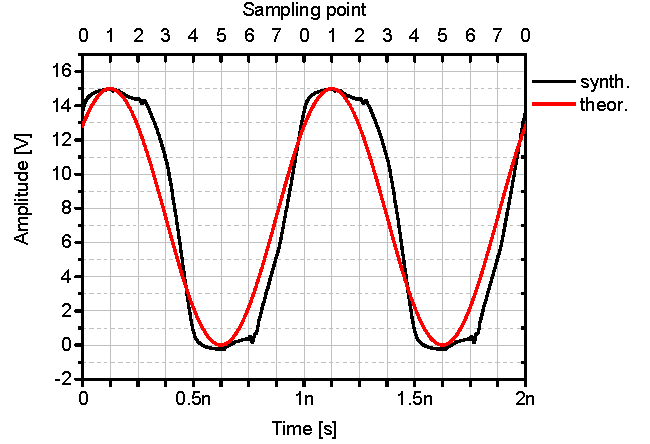
\includegraphics[width=0.75\textwidth]{Vout_SynthVsTheo.pdf}
   \caption{Synthesized sine wave with the theoretical sine wave}
   \label{fig:SineWaveSynthVsTheoretical}
\end{figure}
% 03:12 Uhr 29.04.2016
Although the synthesized signal is clipped and the mentioned distortion came into play, the shape looked like a sine wave.
The \gls{ab:snr} of the synthesized signal was calculated with MatLab and was $SNR = 15$\si{\decibel}.
For a first evaluation of the signal quality after digital-to-analog conversion, the spectra were compared.
The spectrum of a time signal demonstrates the frequency portions which are present in the signal.
As the spectrum of a clear sine wave only consist of a \gls{ab:dc} component and its first harmonic, it was easy to obtain a comparable quantity compared to the synthesized signal.
Figure \ref{fig:SineCompare} highlights the difference between the synthesized and the theoretical sine wave form in more detail.

\begin{figure}[htb!]
	\centering
  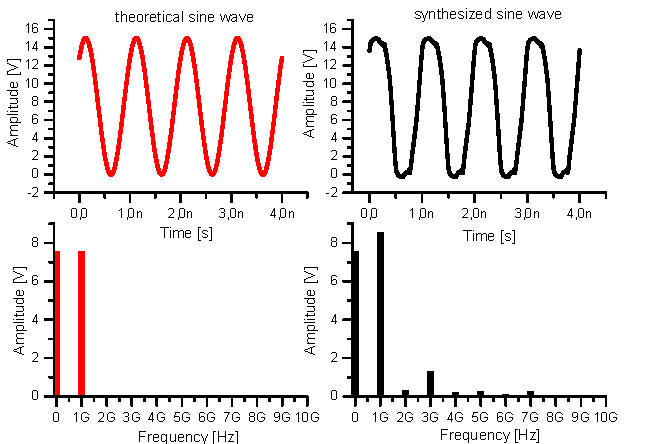
\includegraphics[width=1\textwidth]{SineCompare3.pdf}
	\caption{Comparison between a theoretical and a synthesized sine wave with their spectrum}
	\label{fig:SineCompare}
\end{figure}

On the top left side the theoretical sine wave is plotted in time domain. 
Underneath of it the spectrum presented a frequency portion for the direct component at \SI{0} {\Hz} and a fundamental frequency portion at \SI{1}{\GHz}. 
The spectrum of the synthesized sine wave on the top right side demonstrates a few distortions at higher frequencies.
Beside the direct and fundamental frequency component there were some additional unwanted frequency portions which distorted the signal.
The comparison of the spectra was a good indicator for a first error estimation.
This optical measure made it easy to evaluate the signal quality since the unwanted distortions were clear visible.
At the third harmonic the signal deviates by 14\% from the clear sine, as for the 2nd to 10th harmonic the deviation is up to 7\%.
As already mentioned the calculated \gls{ab:snr} was \SI{15.2}{\decibel} of a theoretical achievable \SI{27}{\decibel}, since this signal was scaled for the full scale.
Compared to a full scale sine wave, a \gls{ab:snr} of \SI{22}{\decibel} could be achieved for a frequency of \SI{1.5}{\giga \hertz} with the presented Riemann Code in equation \ref{eq:RiemannCodeSineWave}.
Figure \ref{fig:SNRSine1.5GHz} demonstrates this synthesized signal with its \gls{ab:snr}.

\begin{figure}[htb]
	\centering
  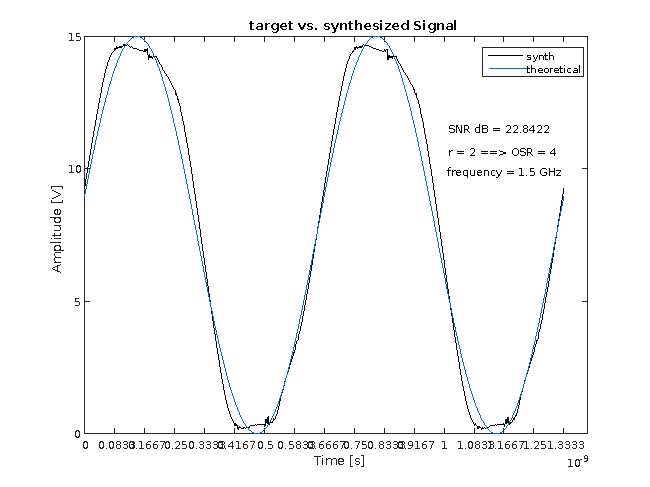
\includegraphics[width=0.9\textwidth]{FullSine15GHz.pdf}
	\caption{calculated SNR for frequency of 1.5 GHz}
	\label{fig:SNRSine1.5GHz}
\end{figure}

Further details on the \gls{ab:snr} calculation for various signals, can be found in appendix \ref{app:snr}.
In addition to tune the amplitude via the absolute sampling intervals, it was also possible to adapt the input control sequence, hence the sequence of chosen slopes to shape the output signal.
The three bit resolution restricted the quantity of different slope combinations to six for synthesizing a sine wave.
Considering only two sampling intervals to construct the rising edge of the positive half sine, the six combinations were: 75, 73, 71, 53, 51 ,31 with respect to the $i_0$ values.
As these relative slopes were used for the rising edge, the counterparts (negative values) represent the falling edge.
The first digit indicated the slope of the first sampling interval and the second digit of the second, respectively. 
These six combinations were plotted in Figure \ref{fig:SameSigBWDifSlope} over two periods for the signal frequency of \SI{3}{\GHz}. 

\begin{figure}[htb!]
	\centering
  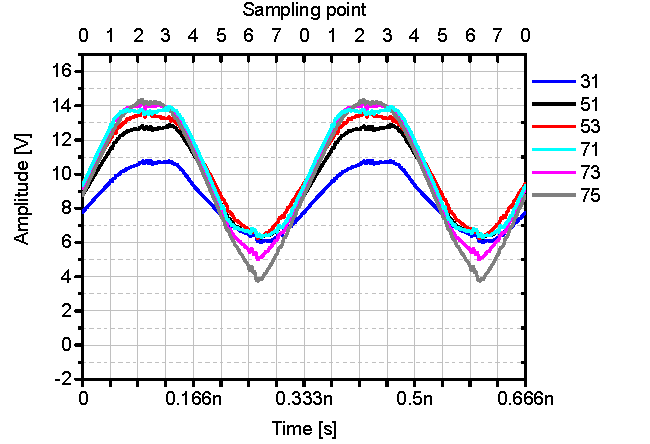
\includegraphics[width=.75\textwidth]{Vout_7sine_SameSigBWdifferent_DifferentSlope.pdf}
	\caption{Signals with the same signal bandwidth \SI{3}{\giga \hertz} but different input control}
	\label{fig:SameSigBWDifSlope}
\end{figure}

Here the effect of the Riemann Code became clear, since the change of the input control will also change the shape of the output signal.
This was utilized to calculate the Riemann Code with an algorithm to fit the output to the desired signal.
The algorithm had to be processed within the settling time of the \gls{ab:dac} to ensure real time conversion.

\subsection{Full wave rectified sine wave generation in the time domain}
In addition to the sine wave, here a full wave rectified sine wave was simulated.
Based on the same approximation principle as demonstrated in figure \ref{fig:RiemannCodeGenerationSineWave}, the corresponding Riemann Code for the rectified sine was generated and is stated in equation \ref{eq:RiemannCodeRectSine}.

%% THIS CORRESPONDS TO 7 5 3 1 -1 -3 -5 -7 
%% SINCE THIS IS ENOUGH TO SYNTHESIZE A PERIOD
\begin{equation}
 000\hspace{.3cm} 001\hspace{.3cm} 010\hspace{.3cm} 011\hspace{.3cm} 100\hspace{.3cm} 101\hspace{.3cm} 110\hspace{.3cm} 111.
\label{eq:RiemannCodeRectSine}
\end{equation}

As the rectified sine wave consisted only of the positive wave for a full period, the oversampling ratio is performed on half of a sine wave.
This resulted in a more precise wave form which resulted in an \gls{ab:osr} of eight (r=3) compared to the full sine wave.
Here the number of slopes used for synthesizing the rising edge was doubled and hence four different slopes could be used.
Therefore the rectified sine wave consisted of eight sampling points, while the corresponding positive half of a sine wave only consisted of four sampling points.
The rectified sine wave exhibited the sequence of all eight different slopes, from the biggest positive to the biggest negative slope.\\
Signals in the frequency range of \SI{500}{\mega \hertz} to \SI{6}{\giga \hertz} were generated and  are demonstrated in Figure \ref{fig:DiffSigBWSameSlope}.

\begin{figure}[htb!]
	\centering
  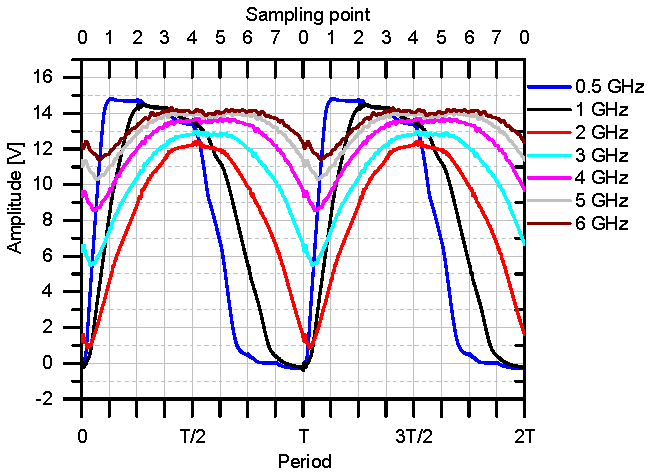
\includegraphics{Vout_halfsine_7531_diff_freq.pdf}
	\caption{Signals with same slope but different signal bandwidth}
	\label{fig:DiffSigBWSameSlope}
\end{figure}

The shapes of the signals with fundamental frequencies \SI{2}{\giga \hertz} to \SI{6}{\giga \hertz} fit very good to a rectified sine..
The issue of signal clipping was the same as mentioned earlier.
This effect was seen in Figure \ref{fig:DiffSigBWSameSlope} for the blue curve which had a fundamental frequency of \SI{500}{\mega \hertz}.
Further investigations on the \gls{ab:snr} were omitted due to the limited scope of this thesis.

\subsection{Triangular wave generation in the time domain}
As the designed circuit should act as a signal generator another signal was synthesized.
A triangular signal was chosen to validate the feasibility of generating arbitrary waveforms.
The wave form of a triangular signal is generated by charging and discharging a capacitor for the same period of time.
All simulations so far, were run with a three bit resolution of the realised circuit.
This three bit resolution represented eight different slopes and therefore for a equally charge and discharge process four different slopes could be used.
These four slopes were +7, +5, +3, +1 for the charging process and their counterparts -7, -5, -3, -1 for discharging.
Hence the sequences of slopes were: 77,55,33 and 11 with respect to $i_0$ values.
Figure \ref{fig:DiffSlopeSameBWTriangular} demonstrates the four different combinations for synthesizing a triangular wave form for \gls{sy:fsignal} = \SI{2}{\giga \hertz}.

\begin{figure}[htb!]
	\centering
  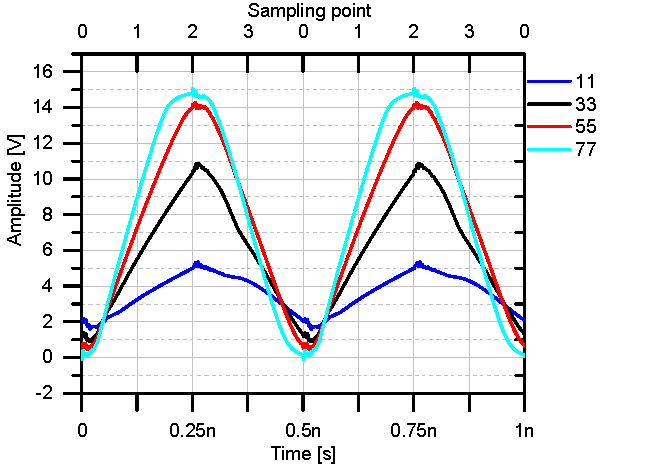
\includegraphics{Vout_triangular_2GHz_diffSlopes.pdf}
	\caption{Triangular signal with same signal bandwidth but different slopes}
	\label{fig:DiffSlopeSameBWTriangular}
\end{figure}

The fundamental frequency was set to \SI{2}{\giga \hertz} representative for the signals with \gls{sy:fsignal} in the frequency range of \SI{500}{\mega \hertz} to \SI{6}{\giga \hertz}.
In this configuration only the wave form for the biggest slope (77; cyan) deviates from the desired signal.
At the sampling point 2 the output capacitance is fully charged which led to an undesirable signal form.
In fact of the high current and long sampling interval, the output capacitor is fully charged.
The problem of not defined reference currents can be observed in the following calculation.
For a reference current $i_0$ of approximately \SI{160}{\milli \ampere}, a capacitance $C$ of \SI{20}{\pico \farad} and a sampling interval $dt$ of \SI{125}{\pico \second} the voltage swing can be calculated as:
\begin{equation}
	dU = \frac{7 i_0*2 dt }{C} = 14 V,
\end{equation}

which fit pretty good to the cyan signal in Figure \ref{fig:DiffSlopeSameBWTriangular}.
Taken the same parameters for the slope of $5 i_0$ it follows a voltage swing of $dU = 10 V$, $dU = 6 V$ and $dU = 2 V$ respectively for $3 i_0$ and $1 i_0$.
As mentioned earlier the problem of not perfectly defined current sources came into play, since this voltage swings could not be observed in Figure \ref{fig:DiffSlopeSameBWTriangular}. 
Representative for the four combinations to synthesize this triangular signal wave form, 
Figure \ref{fig:DiffSigBWSameSlopeTriangular} demonstrates the frequency varying signals from \SI{500}{\mega \hertz} to \SI{6}{\giga \hertz} for a slope of 33.


\begin{figure}[htb!]
	\centering
  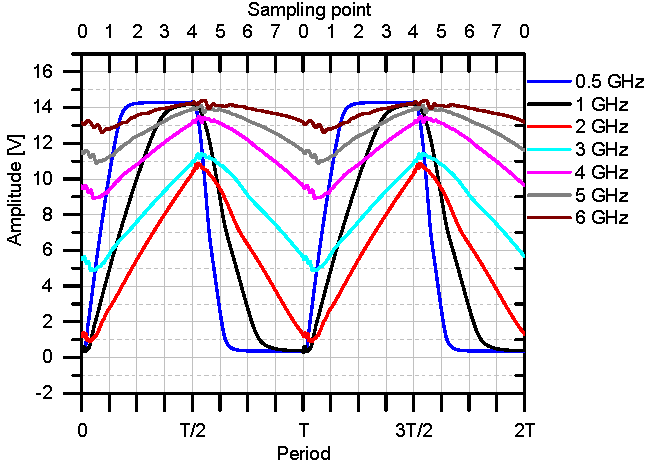
\includegraphics{Vout_triangular_Slope33_diffFreq.pdf}
	\caption{Triangular signal with same slope but different signal bandwidth 3GHz}
	\label{fig:DiffSigBWSameSlopeTriangular}
\end{figure}

%The Code for the generation of the triangular signal at the output is:
%\textbf{this is not the correct code!!}
%\begin{equation}
% 000\hspace{.3cm} 010\hspace{.3cm} 101\hspace{.3cm} 111\hspace{.3cm} 000\hspace{.3cm} 010\hspace{.3cm} 101\hspace{.3cm} 111.
%\end{equation}
%\label{eq:RiemannCodeRectSine}

% short definition of stability, what cause oscillation, how to measure stability -> plot stability circles for the schematic%
\section{Stability analysis of the realised circuit}
To guarantee a proper function of the circuit a short stability analysis was performed.
This analysis was necessary to check if the circuit oscillates.
To prevent the circuit to take damage this oscillation had to be avoided.
It was checked if the \gls{ab:dut} was stable for the whole frequency range used.
Using a S-parameter simulation the complex impedance at various critical points was calculated.
One condition to start an oscillation is a feedback path which existed for the designed circuit.
The driver circuit for the high side switch is connected to the output and hence the feedback is established.
To avoid unwanted oscillation the real part of the complex impedance had to be positive for the whole frequency range.
A basic definition of passive elements were that they have a reflection coefficient magnitude less than unity.
Checking the input reflection coefficient, the values had to be inside the unity circle.
Therefore no negative resistance would be allowed to occur since that can lead to unwanted amplification and oscillation which can damage the circuit \cite{GilmoreR.2003}.
Because the real part of the impedance at all measurement points were positive for the whole frequency range, the circuit seemed to be stable.
The stability check was performed within the \gls{ab:ads} tool. 

\section{Power consumption analysis of the realised circuit}
As the concept is designed for the purpose to implement in mobile communication systems the power consumption is crucial.
Since the energy storage of mobile devices is limited, it is important to get a decent power dissipation for the test circuit.
A short analysis should give an insight to the expected power consumption of the designed test circuit.
Due to the expected switching losses \cite{Quay2014}:
%$ P_{cond} = R_{DS,on}dI_0^2 \propto R_{DS,on} $ \\
\begin{equation}
 P_{sw} = \frac{1}{2} V_{in}I_0(t_{on}+t_{off})f_{sw} \propto f_{sw}
 \label{eq:swtichloss}
\end{equation}

the power consumption scales linear with the switching frequency, here \gls{sy:fsampling}.
Simulations confirmed this assumption for switching the smallest bit of the Riemann Pump.
The used input code was a sequence of alternating bits, since its a different power consumption for switching $+1 i_0$ than for $-1 i_0$.
Switching the high side transistor to the off state results in a leakage current over the high sides driver circuit.
A trade off between switching speed and power consumption resulted.
For an increase in the switching speed, hence an increase of the signal bandwidth, the power consumption also linearly increase.
In addition to this, the power consumption of the driver circuit also increases with the switching speed, as the dimensions of the used components have to be adapted.
The used driver circuit was optimized to reduce the power consumption for a maximum frequency of \SI{100}{\mega \hertz}, as it was implemented in a power application system \cite{MaksimovicPaper}.
In Table \ref{tab:switchloss} the losses are illustrated with the corresponding sampling (switching) frequency of the used configuration.

\begin{table}[ht]
\centering
\begin{tabular}{|l|l|}
\hline
$f_{sampling}$ {[}GHz{]} & $P_{diss}$ {[}W{]} \\ \hline
4                    & 3.982              \\ \hline
8                    & 4.259              \\ \hline
16                   & 4.778              \\ \hline
24                   & 5.011              \\ \hline
32                   & 5.144              \\ \hline
40                   & 5.264              \\ \hline
48                   & 5.354              \\ \hline
\end{tabular}
\caption{Overall power losses for sampling rate}
\label{tab:switchloss}
\end{table}

The used configuration referred to the one bit Riemann Pump consisted of two power transistors, for the high and low side switch, with a gate periphery of \SI{800}{\micro \meter}, four driver transistors each with \SI{200}{\micro \meter} gate periphery and the bias voltages of \gls{sy:vdn} = \SI{-5}{\volt}, \gls{sy:vdp} = \SI{0}{\volt} and \gls{sy:Vdd} = \SI{15}{\volt}.
This configuration can be seen in appendix \ref{app:schematic} on the right hand side.
%As stated in the fundamentals the energy consumption for a dac with 17 ENOB and a sampling rate of 10G will result in several kilo watts, this dac also consumed so much. As the following bits, here power transistors scale with a factor of two it yielded a consumption for 17 bit at 10 G of: sum(2^i), i =0:16 = 131071 i0 = 131071*4W = 400kW --> reference to DAC used in the paper for fig 2.2

\newpage
\section{Proof of concept simulation with existing components}
\label{ch:ProofOfConceptWithExistingComponents}
In the last step a simulation was run which made the concept comparable to the realized circuit. 
The realized circuit was designed with the help of former designed chips.
In this simulation the transistor dimensions were adapted to the dimension of the built demonstrator. 
This should give an insight to the behaviour of the constructed demonstrator.
The detailed modelling and simulation of the designed circuit under real conditions, considering all loss effects would go beyond the scope of this thesis, since no models for the used chips were available.
As the realized demonstrator differs slightly from the presented concept, Figure \ref{fig:democircuit} demonstrates the circuit schematic for one bit.
\begin{figure}[htb!]
	\centering
  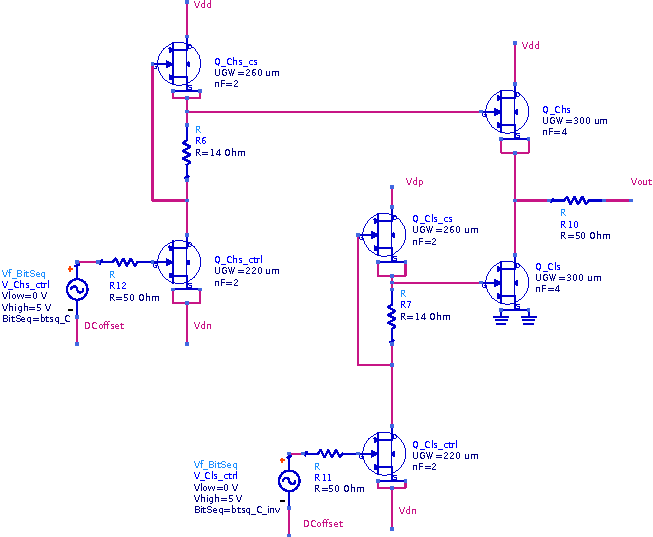
\includegraphics[width=\textwidth]{realizedCircuit_oneBit_DDRi_XY6.pdf}
	\caption{demo circuit}
	\label{fig:democircuit}
\end{figure}

The difference to the presented concept was that no feedback path from the output to the drain of the high side driver circuit existed.
The result of this was that the efficiency was not as good as for the presented concept in chapter \ref{ch:design}.
It is to mention that the transistors for the other bit scales with the factor 2.
The full schematic of the built demonstrator circuit can be seen in Appendix \ref{app:schematicRealizedPump}.
Although the used chips for the demonstrator were designed in a former work, no simulation files were available which made a detailed simulation difficult.
Nevertheless this built circuit acted as expected and a signal could be synthesized, as seen in Figure \ref{fig:sim}.

\begin{figure}[htb!]
	\centering
  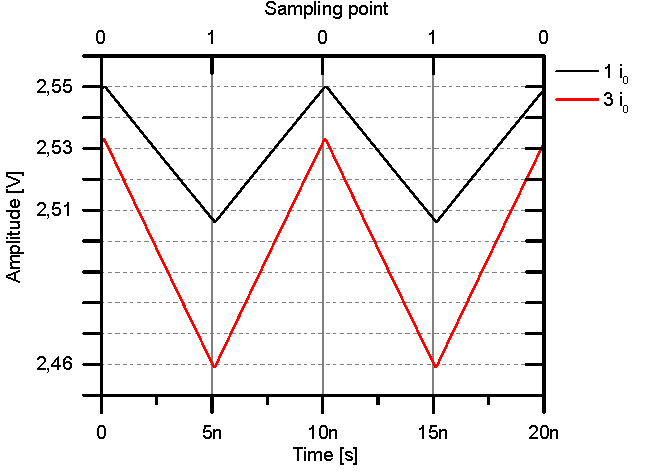
\includegraphics{SimulationForMeasData.pdf}
	\caption{Simulation result for the output voltage using the realized components}
	\label{fig:sim}
\end{figure}

As the measurement of the time signal was performed with an oscilloscope and a probe, the load impedance differs from the concept.
Figure \ref{fig:equivalentprobecircuit} in Chapter \ref{ch:timedomainmeas} presents the equivalent circuit for the measurement.
Considering this, gave the simulation results presented in Figure \ref{fig:sim} which demonstrates the signal generation.
The black signal represents a triangular waveform with a relative slope of $1 i_0$ and the red of $3 i_0$, respectively.
The voltage swing is $0.04 V$ and $0.07 V$ since the probe divides the real voltage with a ratio of 10:1 to avoid any damage of the oscilloscope.
Therefore the real voltage swing is $0.4 V$ and $0.7V$ which fit pretty good to the measured data in chapter \ref{ch:timedomainmeas}.
The simulation is run with the circuit in Figure \ref{fig:democircuit}, a load impedance corresponding to the measurement in Figure \ref{fig:equivalentprobecircuit} in Chapter \ref{ch:timedomainmeas}, \gls{sy:fsampling} of \SI{200}{\mega \hertz} and $V_{dn} = -5V, V_{dp} = 0V, V_{dd} = 5V$.



% As DDRi2C is used, bottom vdp(in na; lowside) = vdd. 
\newpage
\section{Evaluation of the simulation results for the Riemann Pump}
Different wave forms could be synthesized (sine wave, rectified sine, triangular).
The dimension of the used components already limits the bandwidth.
To shift the bandwidth to higher values the transistor dimension have to be bigger and smaller to shift to lower values, respectively.
The signal frequency of \SI{1}{\giga \hertz} represented a lower bound on the frequency range in the used configuration.
With an \gls{ab:osr} of four \gls{sy:fsampling} is eight times \gls{sy:fsignal}.
The smallest achievable current times the smallest sampling time (highest sampling frequency) determine the smallest voltage step achievable.
If the \gls{ab:osr} is increased, the sampling time is decreased and therefore the signal quality is better because we have a more accurate synthesized signal. 
The upper bound of the frequency range is limited to the detectable voltage swing of the amplitude.
In addition to this the components have a unity current gain frequency limit.
Higher frequency means much lower sampling time which can lead to non detectable voltage steps (slopes are not detectable).
Parasitic and loss effects distorted the waveforms.
Since the digital to analog conversion always introduces noise to the signal the fit was not perfect.
The highest \gls{ab:snr} (\SI{32.5}{\decibel}) found was for a sine wave at \SI{6}{\giga \hertz} with an amplitude of $\hat{v} = 1.75 V$, an DC-offset of $V_{DC} = 13 V$ and a phase shift of $\phi = -\pi/8$, see appendix \ref{app:snr}.
There are the \gls{ab:snr} values presented for the seven different signals of Figure \ref{fig:7SignalsSameSlopeInOnePlot} with their corresponding theoretical wave form parameters.
The system is stable.
The stability check was needed to validate that the circuit did not oscillate.
The energy consumption is in the range for base stations and have not reached it yet for mobile devices.
Since the resolution should be in the range of 17 bits.
If the resolution is increased to get a better accuracy, the whole circuit would become more complex and the energy consumption would increase.
If the \gls{ab:osr} is increased to get a better accuracy, the switching frequency is also increased and therefore the energy consumption.
For high switching frequencies the switches have to switch within a few \si{\nano \second} which increase the gate drive current which increase the power loss.
This is the trade off between the shift of the bandwidth (shifting to even higher frequencies is possible but the bandwidth is nearly constant) and power consumption.
The designed test circuit is not optimal with respect to efficiency.
The implemented driver circuit absorbed unexpected leakage currents.\\
Nevertheless the simulation results confirmed the feasibility of the chosen approach.
Some trade-offs in mind and the ability to change some system parameter made it possible to generate some good fitted signal waveforms.